\chapter{Przetwarzanie danych}
\label{chapter:przetwarzanie_danych}

\section{Wczytanie i oczyszczenie danych}

Pierwszym etapem przygotowania danych do użycia w modelu jest ich wczytanie oraz przetworzenie. Zbiór danych z EmoContext zawiera pięć kolumn (rys. \ref{rys:examples_semeval}). W pierwszej kolumnie znajduje się identyfikator, w kolumnach od 2 do 4 zawarty jest docelowy tekst który będzie użyty jako wejście do modelu, a w ostatniej kolumnie znajduje się etykieta emocji. Po wczytaniu danych następuje połączenie trzech kolumn z tekstem w jeden ciąg znaków, oddzielone znakiem specjalnym \textit{EOS} (ang. \textit{end of sentence}). Jest to niezbędna operacja która umożliwi docelowemu modelowi oddzielić trzy wypowiedzi od siebie. Następnie na tak otrzymanym ciągu znaków wykonywane są operacje usuwania powtarzających się znaków interpunkcyjnych (np. \textit{"!!!!"} zostanie zamienione na pojedynczy znak \textit{"!"}). Na końcu wykonywane jest oddzielenie znaków interpunkcyjnych od wyrazów, usunięcie powtarzających się spacji oraz zamiana wszystkich dużych liter na małe.

Jest to wspólny proces dla wszystkich modeli, kolejne etapy zostały podzielone na te zastosowane do architektur korzystających z rekurencyjnych komórek LSTM oraz tych korzystających z architektury BERT. 

\section{Przetwarzanie dla architektur LSTM}

\subsection{Tokenizacja i wyrównanie}

Modele głębokie przetwarzania języka naturalnego nie operują na jawnym tekście w postaci ciągu znaków, tylko na reprezentacji w postaci liczbowej. Do reprezentacji wyrazów używane są słowniki które przechowują wszystkie znane słowa z korpusu uczącego. Do tej zamiany użyta została metoda \texttt{Tokenizer} z pakietu TensorFlow. Klasa ta pozwala na wektoryzację korpusu tekstu, poprzez przekształcenie każdego wyrazu w liczbę całkowitą. Każda z tych liczb odpowiada indeksowi tego słowa w słowniku.

Po przekształceniu każdego słowa w token następuje wyrównanie długości wszystkich przykładów w zbiorze. Przykładowa liczba użyta do wyrównania (ang. \textit{padding}) to 20. Wszystkie przykłady, które mają mniejszą liczbę tokenów, wypełniane są tokenem zerowym aż do osiągnięcia długości 20, a wszystkie przykłady które mają większą liczbę tokenów są skracane od końca. W ten sposób została utworzona macierz danych która może być wykorzystana do użycia w nauce i ewaluacji modeli.

\subsection{Zagłębienia słów}
\label{section:words_embeddings}

W przypadku głębokich sieci neuronowych z rekurencyjnymi komórkami LSTM wysoce efektywne jest użycie zagłębień słów (ang. \textit{words embeddings}) jako wejścia do pierwszej warstwy sieci neuronowej. Osadzanie słów jest przeprowadzone za pomocą mapowania tych słów na wektory liczb rzeczywistych. Reprezentacja słów jako wektory liczb jest rozszerzeniem reprezentacji \textit{jeden z N} (ang. \textit{one hot encodings}), która jest używana w celu zwiększenia wydajności modeli NLP. Jest to także możliwość użycia transferu wiedzy w postaci wstępnie wytrenowanych zagłębień słów jako reprezentacji danych wejściowych. Jednym z algorytmów, który umożliwia stworzenie takiej reprezentacji jest metoda GloVe  \cite{brochier2019global} (ang. \textit{Global Vectors for Word Representation}), stworzona przez zespół z Uniwersytetu Stanford. Udostępniona przez nich macierz umożliwia użycie tej reprezentacji, jako odwzorowanie słów na wektory liczb rzeczywistych. Słowa zmapowane w tej przestrzeni mają zachowane pewne właściwości, odległość między nimi jest powiązana z podobieństwem semantycznym. Na rysunku \ref{rys:visualize_glove} ukazane są przykładowe słowa i zachowane podobieństwo np. między słowami love i beautiful. Sposób uzyskania tej reprezentacji bazuje na współwystępowaniu danych słów w korpusie w otoczeniu które je definiuje. Główną intuicją tego modelu jest założenie, że proporcje prawdopodobieństwa współwystępowania słów mają potencjał do kodowania jakiejś formy znaczenia. Wynikiem tej metody są wektory słów które bardzo dobrze radzą sobie z zadaniami opartymi o podobieństwo, analogię, a także odkrywaniu semantyki emocjonalnej słów i wiele innych wymienionych w pakiecie \textit{word2vec} \cite{mikolov2013efficient}.

\begin{figure}[t]
\centering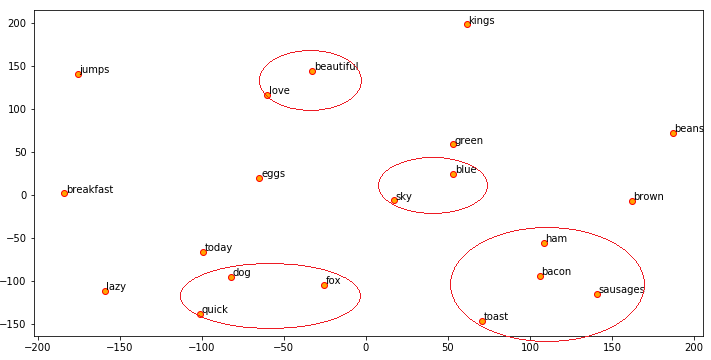
\includegraphics[width=\textwidth]{figures/visualize_glove.png}
\fcmfcaption{Przykładowe słowa w przestrzeni wektorowej GloVe  \cite{brochier2019global}.}\label{rys:visualize_glove}
\end{figure}

\section{Przetwarzanie dla architektur BERT}

Do utworzenia reprezentacji wejściowej dla architektury BERT niezbędne było dostosowanie się do wymagań dla tego modelu. Do przetworzenia tekstu na tokeny użyto klasę \texttt{BertTokenizer} z pakietu \texttt{transformers}. Umożliwia ona zamianę reprezentacji ciągu znaków na tokeny które są mapowane dzięki wbudowanemu słownikowi w architekturę BERT za pomocą algorytmu \textit{WordPiece} \cite{wu2016googles}.

\subsection{Tokenizacja, dodatkowe tokeny i wyrównanie}

Tokenizacja rozkłada się na kilka etapów, jednym z nich jest dodanie specjalnych tokenów oznaczających początek (\textit{[CLS]}) oraz separację (\textit{[SEP]}) kolejnych wypowiedzi, widocznych jako Input na rysunku \ref{rys:bert_token}. Następnie wydzielone tokeny mapowane są na identyfikatory za pomocą wbudowanego słownika. W ten sposób otrzymane reprezentacje zdań zostają wyrównane do danej szerokości i przekazane do wygenerowania maski uwagi o tej samej szerokości co wyrównane zdanie. Ma to na celu wskazanie na których miejscach w zdaniu występują tokeny należące do zdania za pomocą liczby 1. Te tokeny w zdaniu które były sztucznie dodane dla celów wyrównania otrzymują liczbę 0. Tak otrzymana reprezentacja zostanie przekazana na wejście modelu korzystającego z architektury BERT.

\begin{figure}[t]
\centering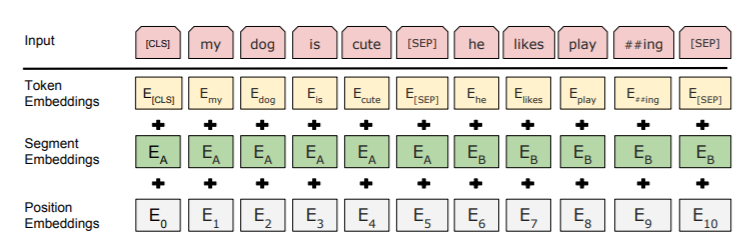
\includegraphics[width=\textwidth]{figures/bert_token.png}
\fcmfcaption{Przykładowe zdanie zamienione na reprezentację BERT \cite{devlin2018bert}.}\label{rys:bert_token}
\end{figure}